% \chapter{Trabajo}

% Preface
% \note{Soy un estudiante italiano en Erasmus. Hablo espanol bastante bien, pero me resulta mas natural escribir en ingles; sin embargo, decidi escribir en espanol para practicar, con la ayuda de algunos traductores cuando era necesario. Si hay algo mal escrito o poco claro, estoy a disposicion para cualquier aclaracion.}

\begin{figure}[htbp]
   \centering
   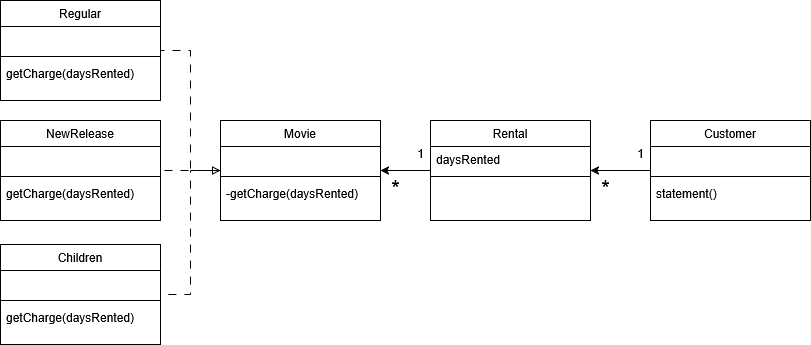
\includegraphics{images/ACG_Practica2.drawio.png}
   \caption{Diagrama de clases}
   \label{fig:ACG_Practica2.drawio}
\end{figure}

\lstset{language=Java}
\begin{lstlisting}[caption={RentalTest.java}]
   package Principal;
   import static org.junit.jupiter.api.Assertions.*;
   
   import org.junit.jupiter.api.BeforeAll;
   import org.junit.jupiter.api.Test;
   
   public class RentalTest {
      // Declaramos variables Rental, Customer y Movie
      private static Movie movieRegular;
      private static Movie movieNewRelease;
      private static Movie movieChildren;
      
      private static Rental rentalRegular;
      private static Rental rentalNewRelease;
      private static Rental rentalChildren;
      
      private static Customer customer1;
      private static Customer customer2;
   
   /**
    * Dado que alli solo estamos leyendo las istancias en las pruebas,
    * sin alterar el estado interno, BeforeAll parece mas apropiado que
    * BeforeEach, que sin embargo garantizaria el aislamiento de las pruebas.
    * 
    *  */
   @BeforeAll
   public static void setUp() throws Exception {
       // Creamos peliculas usando los constructores directamente
       movieRegular = new RegularMovie("Matrix");
       movieNewRelease = new NewReleaseMovie("Avatar 2");
       movieChildren = new ChildrensMovie("Toy Story");
       
       // Creamos alquileres
       rentalRegular = new Rental(movieRegular, 3);
       rentalNewRelease = new Rental(movieNewRelease, 2);
       rentalChildren = new Rental(movieChildren, 5);
       
       // Creamos clientes
       customer1 = new Customer("Miguel");
       customer2 = new Customer("Ana");
   }
      
      @Test
      public void testMovies() {
          // Comprobamos que el nombre de las peliculas creadas es correcto
          assertEquals("Matrix", movieRegular.getTitle());
          assertEquals("Avatar 2", movieNewRelease.getTitle());
          assertEquals("Toy Story", movieChildren.getTitle());
          
          // Comprobamos que el codigo del precio de las peliculas es correcto
          assertEquals(Movie.PriceCodes.Regular, movieRegular.getPriceCode());
          assertEquals(Movie.PriceCodes.NewRelease, movieNewRelease.getPriceCode());
          assertEquals(Movie.PriceCodes.Childrens, movieChildren.getPriceCode());
      }
      
      @Test
      public void testCustomers() {
          // Comprobamos que los clientes se han creado con el nombre correcto
          assertEquals("Miguel", customer1.getName());
          assertEquals("Ana", customer2.getName());
      }
      
      @Test
      public void testRentals() {
          // Comprobamos que la pelicula asociada al alquiler es correcta
          assertSame(movieRegular, rentalRegular.getMovie());
          assertSame(movieNewRelease, rentalNewRelease.getMovie());
          assertSame(movieChildren, rentalChildren.getMovie());
          
          // Comprobamos que los dias asociados a cada alquiler son correctos
          assertEquals(3, rentalRegular.getDaysRented());
          assertEquals(2, rentalNewRelease.getDaysRented());
          assertEquals(5, rentalChildren.getDaysRented());
      }
      
      @Test
      public void testStatement() {
          // Anadimos los alquileres a uno de los clientes
          customer1.addRental(rentalRegular);
          customer1.addRental(rentalNewRelease);
          customer1.addRental(rentalChildren);
          
          // Obtenemos el string que devuelve statement()
          String result = customer1.statement();
          
          // Calculamos manualmente los importes esperados
          // Construimos el string que esperamos debe devolver statement()
          String expected = "Rental record for Miguel\n" +
                           "\tMatrix\t3.5\n" +
                           "\tAvatar 2\t6.0\n" +
                           "\tToy Story\t4.5\n" +
                           "Amount owed is 14.0\n" +
                           "You earned 4 frequent renter points.";
          
          // Comprobamos que statement() ha devuelto lo mismo que esperabamos
          assertEquals(expected, result);
      }
   
      @Test
      public void testGetCharge(){
          // Comprobamos que el precio que devuelve getCharge de los
          // alquileres que hemos creado es el que hemos calculado
          // a mano que debe ser
          
          // Regular: 2 + (3-2)*1.5 = 3.5
          assertEquals(3.5, rentalRegular.getCharge(), 0.01);
          
          // NewRelease: 2*3 = 6.0
          assertEquals(6.0, rentalNewRelease.getCharge(), 0.01);
          
          // Children: 1.5 + (5-3)*1.5 = 4.5
          assertEquals(4.5, rentalChildren.getCharge(), 0.01);
      }
   
      @Test
      public void testGetFrequentRenterPoint(){
          // Comprobamos que los puntos que devuelve getFrequentRenterPoint
          // de los alquileres que hemos creado es el que hemos calculado
          // a mano que debe ser
          
          // Regular: 1 punto independientemente de los dias
          assertEquals(1, rentalRegular.getFrequentRenterPoint());
          
          // NewRelease: 2 puntos si el alquiler es > 1 dia
          assertEquals(2, rentalNewRelease.getFrequentRenterPoint());
          
          // Children: 1 punto independientemente de los dias
          assertEquals(1, rentalChildren.getFrequentRenterPoint());
          
          // Creamos un nuevo alquiler de NewRelease con 1 dia para comprobar el caso limite
          Rental rentalNewRelease1Day = new Rental(movieNewRelease, 1);
          assertEquals(1, rentalNewRelease1Day.getFrequentRenterPoint());
      }
   }
\end{lstlisting}

\begin{lstlisting}[caption={Customer.java}]
   package Principal;

   import java.util.ArrayList;
   import java.util.List;
   import java.io.Console;
   import java.util.*;
   
   public class Customer {
   
       private String name;
       private List<Rental> rentals = new ArrayList<Rental>();
   
       public Customer(String name) {
           this.name = name;
       }
   
       public String getName() {
           return name;
       }
   
       public void addRental(Rental rental) {
           rentals.add(rental);
       }
   
       public String statement() {
           double totalAmount = 0;
           int frequentRenterPoints = 0;
           Iterator<Rental> iteradorRentals = rentals.iterator();
   
           String result = "Rental record for " + name + "\n";
   
           while (iteradorRentals.hasNext()) {
               Rental each = iteradorRentals.next();
   
               frequentRenterPoints += each.getFrequentRenterPoint();
   
               result += "\t" + each.getMovie().getTitle() + "\t" + Double.toString(each.getCharge()) + "\n";
   
               totalAmount += each.getCharge();
           }
   
           result += "Amount owed is " + Double.toString(totalAmount) + "\n";
           result += "You earned " + Integer.toString(frequentRenterPoints) + " frequent renter points.";
           return result;
       }
   }
   
\end{lstlisting}

\begin{lstlisting}[caption={Rental.java}]
   package Principal;

   public class Rental {
   
       private Movie movie;
       private int daysRented;
   
       public Rental(Movie movie, int daysRented) {
           this.movie = movie;
           this.daysRented = daysRented;
       }
   
       public Movie getMovie() {
           return movie;
       }
   
       public int getDaysRented() {
           return daysRented;
       }
   
       public double getCharge() {
           return movie.getCharge(daysRented);
       }
   
   
       public int getFrequentRenterPoint() {
           if ((movie.getPriceCode() == Movie.PriceCodes.NewRelease) &&
                   (daysRented > 1)) {
               return 2;
           } else
               // no extra point
               return 1;
       }
   
   }   
\end{lstlisting}

\begin{lstlisting}[caption={Movie.java}]
   package Principal;

   public abstract class Movie {
   
       public enum PriceCodes {
           Regular, NewRelease, Childrens
       }
       
       private String title;
   
       public Movie(String title) {
           this.title = title;
       }
   
       public String getTitle() {
           return title;
       }
       
       public void setTitle(String title) {
           this.title = title;
       }
       
       // Metodo abstracto que deben implementar las subclases
       public abstract double getCharge(int daysRented);
       
       // Metodo de puntos de fidelidad - aplicacion por defecto
       public int getFrequentRenterPoints(int daysRented) {
           return 1;
       }
       
       // Por compatibilidad con el codigo existente
       public abstract PriceCodes getPriceCode();
   }
   
\end{lstlisting}

\begin{lstlisting}[caption={RegularMovie.java}]
   package Principal;

   public class RegularMovie extends Movie {
       
       public RegularMovie(String title) {
           super(title);
       }
       
       @Override
       public double getCharge(int daysRented) {
           double result = 2;
           if (daysRented > 2) {
               result += (daysRented - 2) * 1.5;
           }
           return result;
       }
       
       @Override
       public PriceCodes getPriceCode() {
           return PriceCodes.Regular;
       }
   }
\end{lstlisting}

\begin{lstlisting}[caption={NewReleaseMovie.java}]
   package Principal;

   public class NewReleaseMovie extends Movie {
       
       public NewReleaseMovie(String title) {
           super(title);
       }
       
       @Override
       public double getCharge(int daysRented) {
           return daysRented * 3;
       }
       
       @Override
       public int getFrequentRenterPoints(int daysRented) {
         // 2 puntos por alquileres de mas de 1 dia
         return daysRented > 1 ? 2 : 1;
       }
       
       @Override
       public PriceCodes getPriceCode() {
           return PriceCodes.NewRelease;
       }
   }
\end{lstlisting}

\begin{lstlisting}[caption={ChildrensMovie.java}]
   package Principal;

   public class ChildrensMovie extends Movie {
       
       public ChildrensMovie(String title) {
           super(title);
       }
       
       @Override
       public double getCharge(int daysRented) {
           double result = 1.5;
           if (daysRented > 3) {
               result += (daysRented - 3) * 1.5;
           }
           return result;
       }
       
       @Override
       public PriceCodes getPriceCode() {
           return PriceCodes.Childrens;
       }
   }
\end{lstlisting}
